\pagebreak  % Fin de numeración romana
\cleardoublepage
\pagestyle{headings}
\pagenumbering{arabic}

\chapter{Introducción}
%
El actual entorno global en el ámbito de la tecnología insta a los desarrolladores a \ldots

\section{Definiciones}
Un sistema empotrado (\textsf{S.E.}) es \ldots



\section{Antecedentes}
El resultado de combinar los recursos hardware FPGA\nomenclature{FPGA}{Field Programable Gate Array} y software \ldots

La figura \ref{fig_plat_hw} muestra un esquema simplificado de una plataforma hardware usando la topología de bus.

\begin{figure}[h]
  \centering
  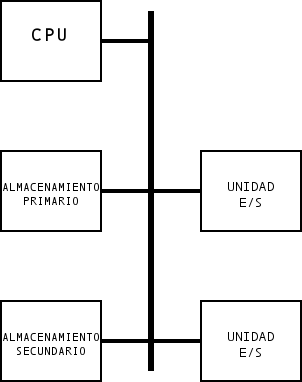
\includegraphics[width=5cm]{fig/plataforma-hw.png} 
  \caption[Esquema estructural de una plataforma hardware.]%
  {Esquema estructural de una plataforma hardware.}
  \label{fig_plat_hw}
\end{figure}

\section{Planteamiento del problema}
Esta tesis pretende \ldots

Para ello es necesario implementar funciones hardware como las mostradas en el siguiente listado.

\begin{center}
\begin{minipage}{10cm}
\lstset{%
	numbers=left, %
	numberstyle=\tiny, %
	stepnumber=1, %
	numbersep=10pt, %
	language=C,%
	basicstyle=\footnotesize
}
\begin{lstlisting}[caption={[Ejemplo de operación 1]Ejemplo de operación para el modelo de ejecución de una función hardware con paso de argumentos por valor.}, label=hw-fun-val-ej]
#include <stdio.h>
...
#include "hard_func.h"

//Def. del prototipo
int HW_FUN (int A, int B, char op); 

int main() {
...
result = HW_FUN(x, y, op);
...
}
\end{lstlisting}
\end{minipage}
\end{center}

El segundo modelo se aplica a \ldots

El listado \ref{hw-fun-ref-ej} muestra un ejemplo de este tipo de funciones.

\begin{center}
\begin{minipage}{10cm}
\lstset{%
	numbers=left, %
	numberstyle=\tiny, %
	stepnumber=1, %
	numbersep=10pt, %
	language=C,%
	basicstyle=\footnotesize
}
\begin{lstlisting}[label=hw-fun-ref-ej, caption={[Ejemplo de operación 2]Ejemplo de operación para el modelo de ejecución de una función hardware con paso de argumentos por referencia.}]
#include <stdio.h>
...
#include "hard_func.h"

// Def. del prototipo
struct *HW_FUN (struct *A, struct *B); 

int main() {
...
data = HW_FUN(data1_ptr, data2_ptr);
...
}
\end{lstlisting}
\end{minipage}
\end{center}

La figura \ref{main-sch} muestra el esquema general de interacción entre hardware y software para el uso de funciones hardware.

\begin{figure}[h!]
  \centering
  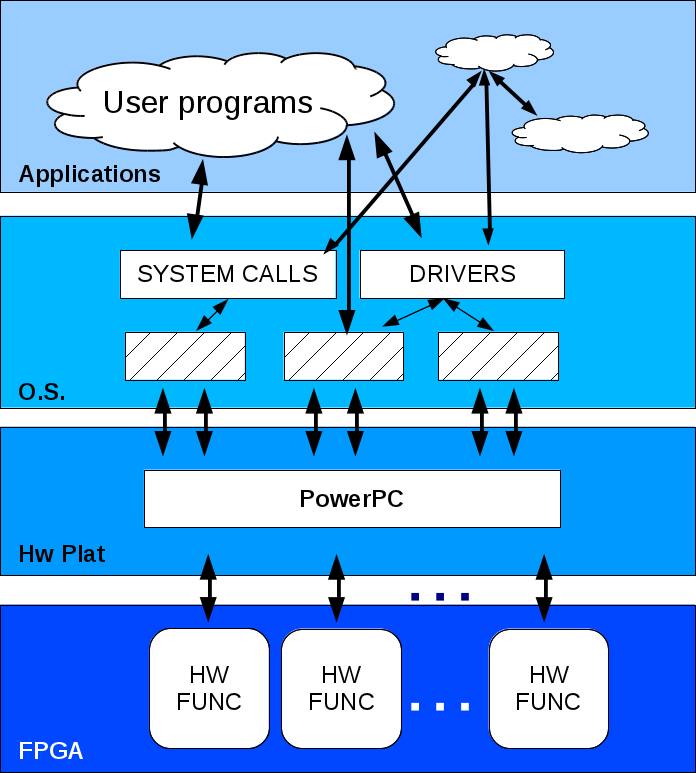
\includegraphics[width=10cm]{fig/main-sch.png} 
  \caption {Esquema de operación hardware/software.}
  \label{main-sch}
\end{figure}



\section{Objetivos}
%Esta sección describe el objetivo general y los objetívos específicos de esta tesis.
%
\subsection{Objetivo general}
\noindent \paragraph{Metodología para el desarrollo de funciones hardware para bibliotecas estáticas.}

\subsection{Objetivos específicos}
\begin{itemize}
\item Obj uno.
\item Obj dos.
\item Obj tres.
\item Obj cuatro.
\end{itemize}

\section{Justificación}
El uso de sistemas \ldots

\subsection{Beneficios esperados}
Esta tesis pretende generar \ldots

\subsection{Alcances y límites}
En este trabajo se pretende \ldots pero sólo utiliza \ldots aunque es posible implementar \ldots

\section{Organización de la tesis}

\begin{description}

\item[Capítulo 1] inicia con una introducción a ...

\item[Capítulo 2] contiene ... 

\item[Capítulo 3] describe ...

\item[Capítulo 4] contiene...

\item[Capítulo 5] contiene los resultados de ...

\end{description}

